\documentclass[a4paper,12pt]{article}
\usepackage{graphicx}
\usepackage{float}
\usepackage{listings}
\usepackage{amsmath}
\usepackage{hyperref}
\graphicspath{{figures/}}
\setlength{\parindent}{0pt}

\begin{document}

    \title{Computational Biomaterials and Biomechanics\\[1ex]
    \Large Intravoxel analysis of clinical CT scan}
    \author{Robin Steiner (11778873)}
    \date{\today}
    \maketitle

    \thispagestyle{empty}
    \newpage

    \tableofcontents

    \newpage

    \section{Introduction}\label{sec:introduction}
    This report discusses the application of computational techniques to analyze a clinical CT scan of a vertebrae.
    The basis is a dataset which assigns frequency counts to grey values within the range of 0 to 256.
    The report will discuss several steps necessary to gain insight on the longitudinal elastic modulus in the bone include plotting a histograms of grey values, generating a probability density function, identifying characteristic grey values, assessing vascular porosity, and creating a histogram for voxel-specific longitudinal elastic modulus in bony regions.
    All results and plots where generated using \texttt{MATLAB}.

    \section{Solution to the Tasks}\label{sec:solution-to-the-tasks}

    \subsection{Histogram of the Grey Values}\label{subsec:histogram-of-the-grey-values}

    First we plot the histogram of the CT dataset of the vertebrae.
    The result can be seen in Figure~\ref{fig:histogram}
    \begin{figure}[h]
        \centering
        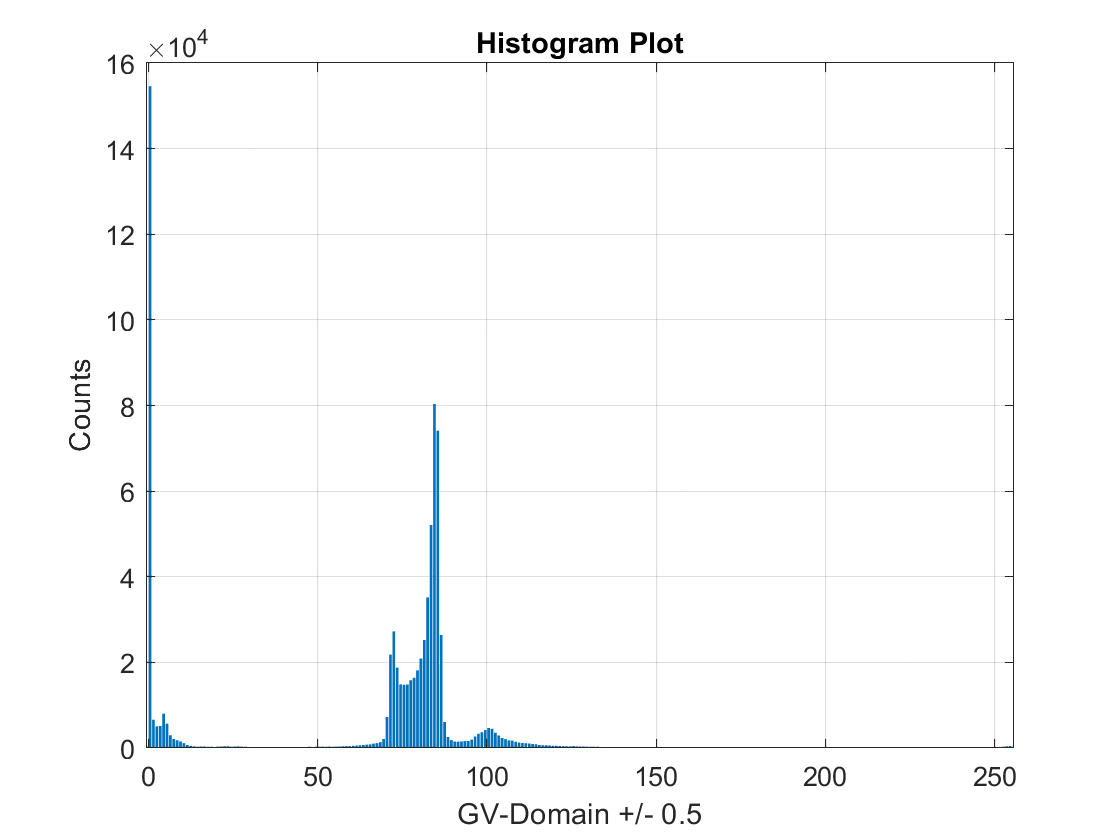
\includegraphics[width=0.8\textwidth]{histogram}
        \caption{Histogram of the grey values}
        \label{fig:histogram}
    \end{figure}

    As we can see, besides the complex between the grey values from 50 to 150, which represent the vertebrae, there is also a big amount of grey values close to zero.
    This indicates that a large part of the scan must have been air.

    \subsection{Probability Density Function}\label{subsec:probability-density-function}
    The next step is to normalize the data by the total counts in the dataset, this gives us the probability density function, which can be seen in Figure \ref{fig:PD}.
    \begin{figure}[h]
        \centering
        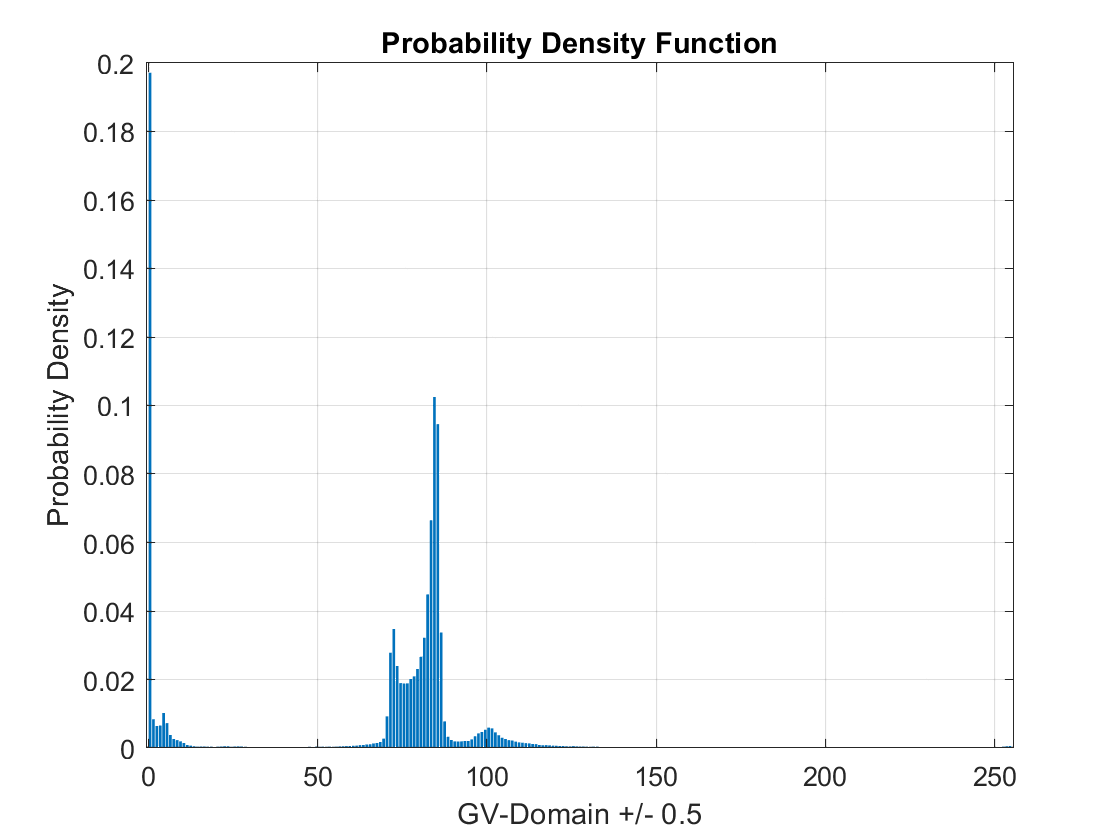
\includegraphics[width=0.8\textwidth]{PD}
        \caption{Probability Density Function of the grey values}
        \label{fig:PD}
    \end{figure}

    \subsection{Identifying Characteristic Grey Values}\label{subsec:identifying-characteristic-grey-values}
    From this probability density function we can identify four characteristic grey values which represent the vertebrae:
    \begin{enumerate}
        \item $GV_{fat} = (72.5, 0.0347)$
        \item $GV_{soft} = (84.5, 0.1025)$
        \item $GV_{thr} = (91.5, 0.0019)$
        \item $GV_{max} = (166.5, 0)$
    \end{enumerate}

    \vspace{10pt}
    $GV_{fat}$ is identified, by finding the first maxima of the relevant section of the probability density function.
    It is associated with fat tissue.
    Likewise, $GV_{soft}$ represents the second maxima and is associated with soft tissue.
    $GV_{thr}$ is the dip (minima) after $GV_{soft}$ and marks the start of the region of the probability density function which represents the bone.
    Finally, $GV_{max}$ represents the highest grey value that can be attributed to the vertebrae.
    It is the first grey value after $GV_{thr}$ which exhibits a probability of zero.

    \vspace{10pt}
    All the values where obtained using code and are plotted in Figure~\ref{fig:PD_with_special_points}
    \begin{figure}[h]
        \centering
        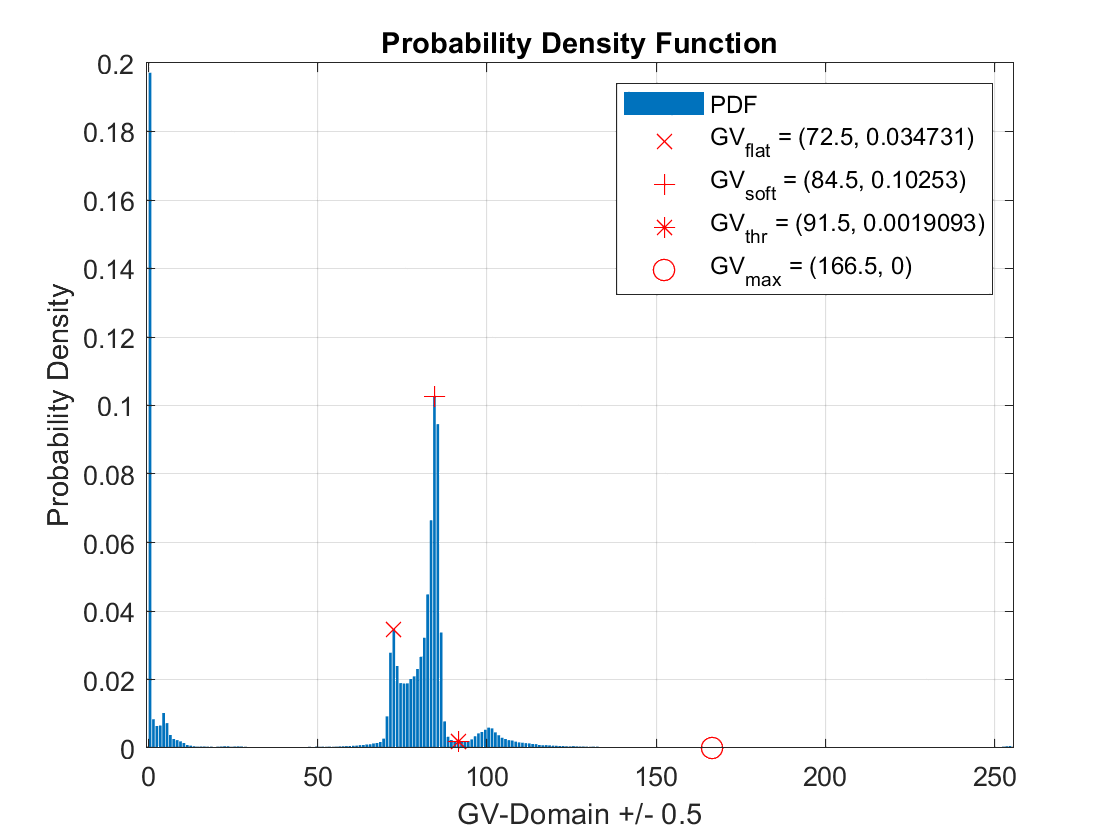
\includegraphics[width=0.8\textwidth]{PD_with_special_points}
        \caption{Probability Density Function with specific grey values describing the vertebrae}
        \label{fig:PD_with_special_points}
    \end{figure}

    \subsection{Vascular Porosity}\label{subsec:vascular-porosity}
    Next we consider $GV_{soft}$ as being relevant for the vascular porosity.
    We calculate the probability density function for the vascular porosity using the averaging rule:
    \[
        GV = \sum_{i=1}^{N_C} GV_i \times f_i
    \]

    combining this with voxel partitioning rules for the cortical shell we obtain the following system of equations:
    \begin{gather*}
        \frac{{l_1}}{{l_{voxel}}} \times GV_{ev} + \left(1 + \frac{{l_1}}{{l_{voxel}}}\right) \times GV_{soft} = GV_{max}\\
        \frac{{l_2}}{{l_{voxel}}} \times GV_{ev} + \left(1 + \frac{{l_2}}{{l_{voxel}}}\right) \times GV_{soft} = GV_{max-1}\\
        l_1 + l_2 = l_{cort},
    \end{gather*}
    with $GV_{ev}$ being the grey value associated with the extravascular tissue. \cite{blanchard2016patient}

    \vspace{10pt}
    Solving this system we get:
    \[
        GV_{ev} = \frac{{l_{voxel}}}{l_{cort}} \times (GV_{max} + GV_{max-1} - 2GV_{soft}) + GV_{soft}\\
    \]
    $GV_{max-1}$ is defined as the densest neighbor of $GV_{max-1}$.
    Its value is taken from literature as $GV_{max-1} = 156$
    Similarly we take the values for the width of the cortical shell $l_{cort} = 0.23\:mm$ and the width of the voxel $l_{voxel} = 0.324\: mm$ from literature~\cite{blanchard2016patient}
    Calculating this for our previously found $GV_{max}$, and $GV_{soft}$ we get $GV_{ev} = 300.53$

    \vspace{10pt}
    Finally, we are interested in the vascular porosity $\phi_{vas}$ of the bony region, which can be obtained with:
    \[
        \phi_{vas} = \frac{{\mu_{macro} - \mu_{ev}}}{{\mu_{H2O} - \mu_{ev}}}\\
    \]
    We can assume a linear relation between the grey value and the attenuation coefficient and therefore use the previously found grey value of the extravascular tissue directly.
    Additionally, we can replace $\mu_{H2O}$ with $GV_{soft}$, since we can assume similar grey values for them. \cite{blanchard2016patient}
    Since we are only interested in the vascular porosity of the bone, we will use the grey values in the region between $GV_{thr}$ and $GV_{max}$, which we assume to be the bony part.
    Doing all this we get:
    \[
        \phi_{vas} = \frac{{GV_{bone} - GV_{ev}}}{{GV_{soft} - GV_{ev}}}\\
    \]

    To get the probability density function for the vascular porosity we multiply the result with 100.
    The final plot can be seen in Figure~\ref{fig:vascular_porosity}.

    \begin{figure}[h]
        \centering
        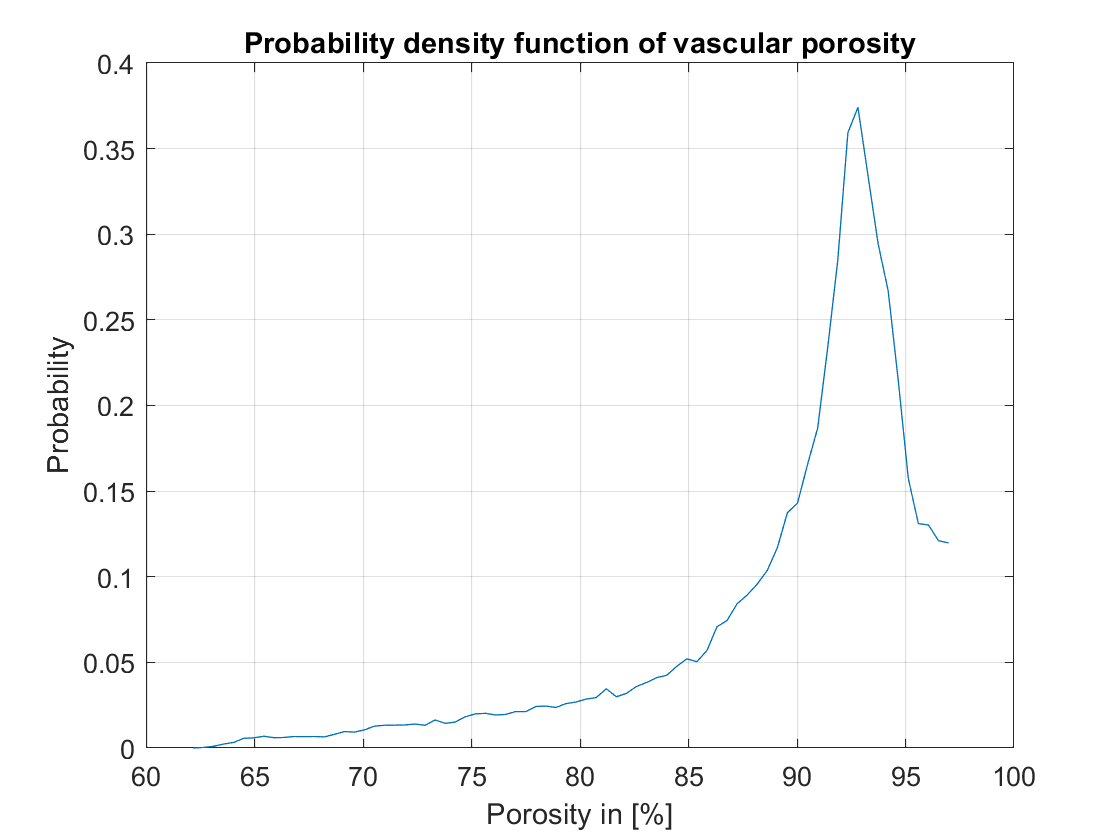
\includegraphics[width=0.8\textwidth]{vascular_porosity}
        \caption{Probability Density Function with specific grey values describing the vertebrae}
        \label{fig:vascular_porosity}
    \end{figure}

    \subsection{Longitudinal Elastic Modulus}\label{subsec:longitudinal-elastic-modulus}
    Lastly we want to find a histogram for the voxel-specific longitudinal elastic modulus in the bony region of the vertebrae.
    For this we utilize a function which calculates the stiffness matrices for a given porosity value.
    The result was inverted and the longitudinal Young's modulus was extracted from the matrix.

    \[
        E_{macro,3} = \frac{1}{C^{-1}_{macro,3333}}
    \]

    Doing this for all the previously obtained vascular porosities, we finally get the plot shown in Figure~\ref{fig:youngs_moduls}

    \begin{figure}[h]
        \centering
        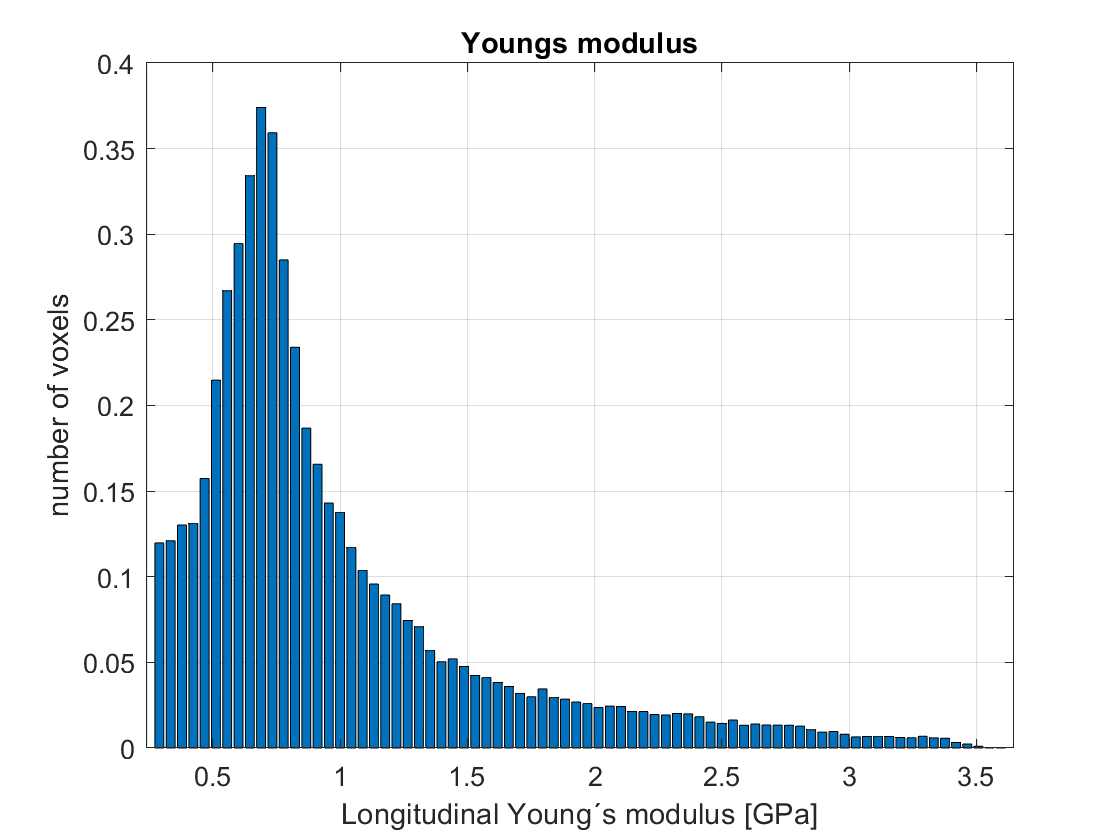
\includegraphics[width=0.8\textwidth]{youngs_moduls}
        \caption{Probability Density Function with specific grey values describing the vertebrae}
        \label{fig:youngs_moduls}
    \end{figure}


    \section{Conclusion}\label{sec:conclusion}

    The grey values obtained in the Section~\ref{subsec:identifying-characteristic-grey-values} are very similar to what was found in~\cite{blanchard2016patient}:

    \begin{table}[h]
        \centering
        \begin{tabular}{lcccc}
            \hline
            \textbf{Source}  & $GV_{fat}$ & $GV_{soft}$ & $GV_{thr}$ & $GV_{max}$ \\
            \hline
            Our Results      & 72.5       & 84.5        & 91.5       & 166.5      \\
            Blanchard et al. & 72         & 84          & 93         & 164        \\
            \hline
        \end{tabular}
    \end{table}

    This is expected considering the same anatomical structure (vertebrae) wa analyzed.

    \vspace{10pt}
    In Section~\ref{subsec:vascular-porosity}, we found the grey value of the extravascular tissue to be $GV_{ev} = 300.53$.
    This again it very close to the result from Blanchard et al. \cite{blanchard2016patient}, where $GV_{ev}$ was found to be $298$.
    This grey value was then used to further calculate the vascular porosity of the bony region of our sample.
    The calculated porosity spans between ~62\% and ~97\%.
    This is because the calculations were performed on a region limited to the grey values representing the bone, so between $GV_{thr}$ and $GV_{max}$.

    \vspace{10pt}
    The Young's modulus plot was generated using the provided function

    \vspace{1pt}
    \texttt{hom\_exvas\_to\_macro}.
    The input porosity values were those calculated in Section~\ref{subsec:vascular-porosity} for the bony region.
    Therefore, the Young's modulus values plotted alongside their corresponding voxel counts pertain solely to the bony region within the CT scan.
    The observed modulus values range from approximately 0.2 GPa to 3.5 GPa.

    \newpage


    \section{References}\label{sec:references}
    \begingroup
    \renewcommand{\section}[2]{}
    \bibliography{refs}
    \bibliographystyle{plain}
    \endgroup

\end{document}
